\begin{boxA}
    برای این تمرین ابتدا مقادیر متغیرهای
    \lr{b}
    و 
    \lr{k}
    را با هم در پوشه‌های جداگانه مقایسه کردم و سپس به ارزیابی بهترین‌ها پرداختم.

    برای مقایسه بین پارامترهای مختلف 
    \lr{b}
    و
    \lr{k}
    اسکریپت‌هایی نوشتم که 
    نتایج 
    حالات مختلف را در فایل
    ‌های متناظر می‌نویسیم و سپس با معیارهای ذکر شده به ارزیابی می‌پردازیم.
\end{boxA}


\begin{figure}[h]
\centering
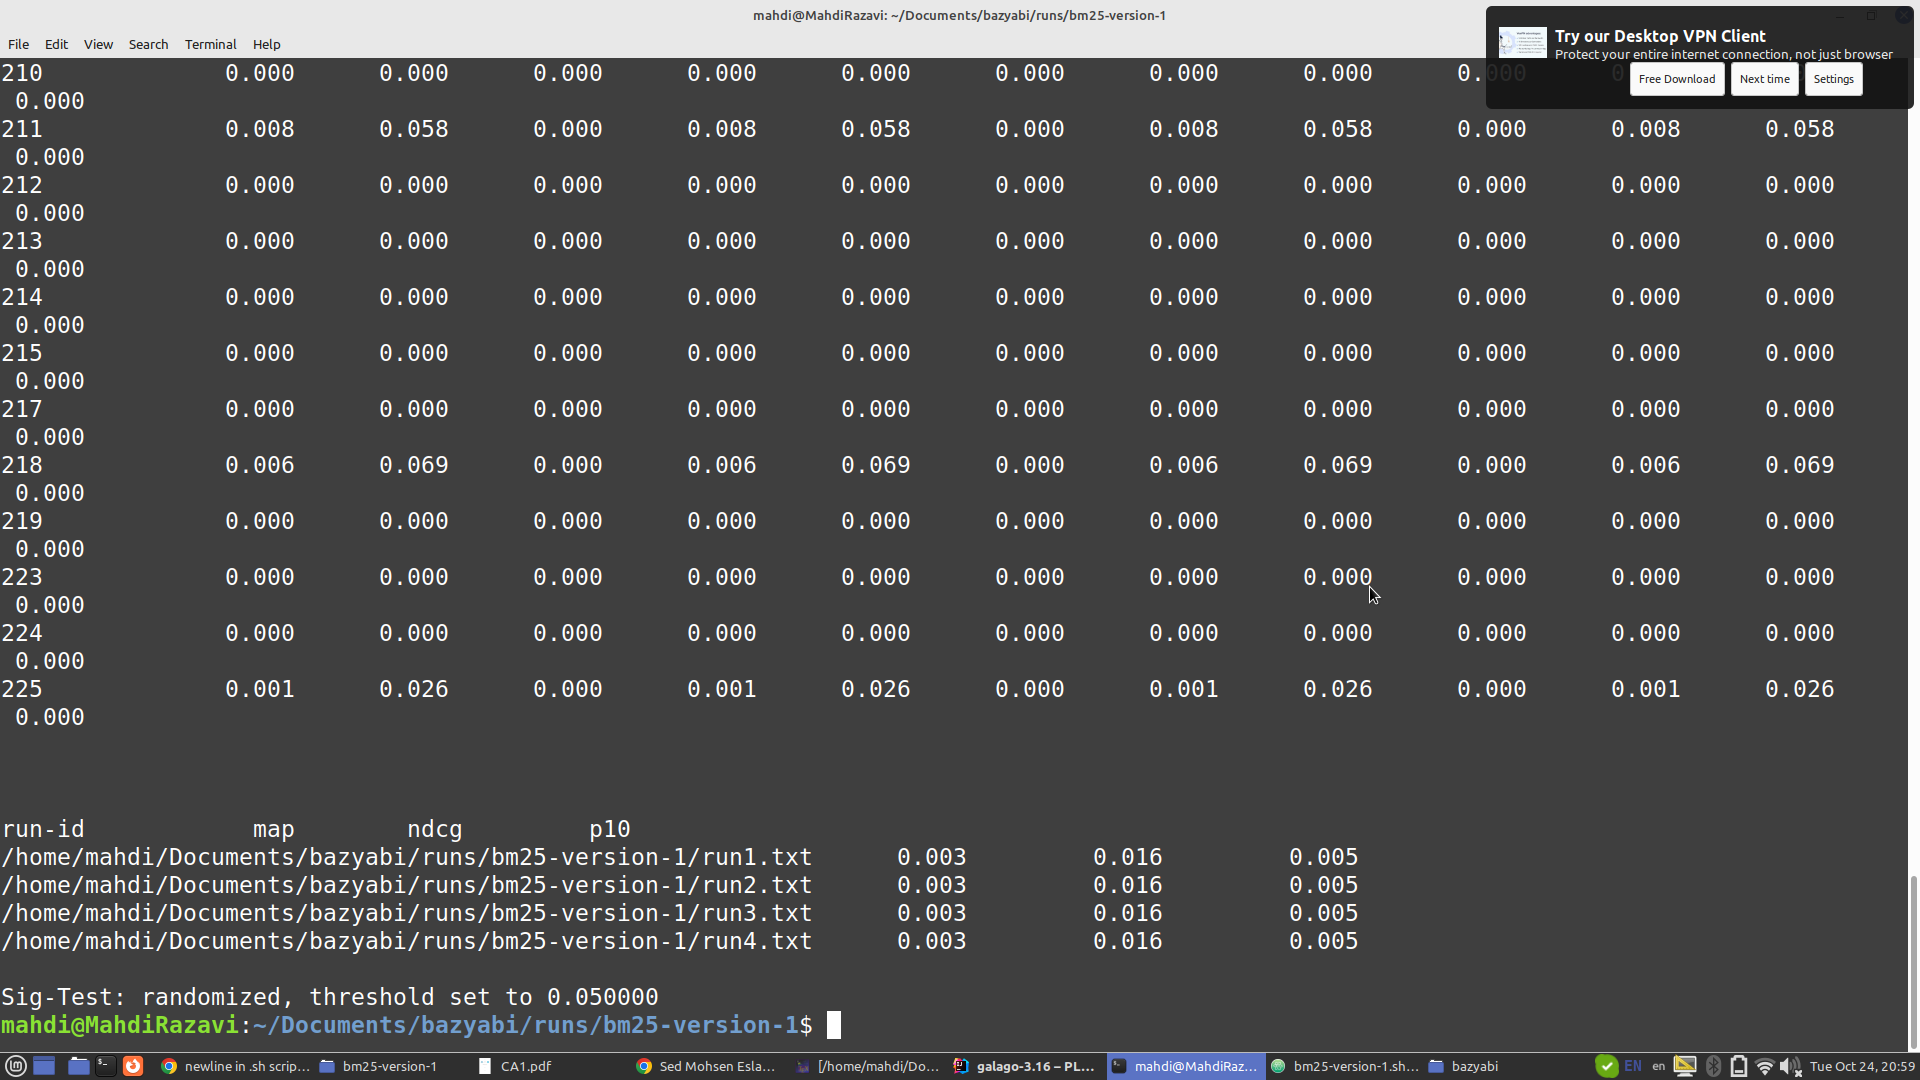
\includegraphics[width=0.8\textwidth]{IR1/images/V1.png}
% \caption{ت هستند.}
\caption{تابع امتیازدهی اول}
\end{figure}

\begin{boxM}
    با توجه به این که تابع اول مستقل از پارامترهای ذکر شده هستند ، در نتیجه نتایج کاملا مشابه هم خواهد بود و نتایج به میزان منحصربفرد بودن 
    یا همان
    \lr{IDF}
    عبارات مشترک متن و پرس‌وجو خواهد بود.
\end{boxM}

\newpage

\begin{figure}[h]
\centering
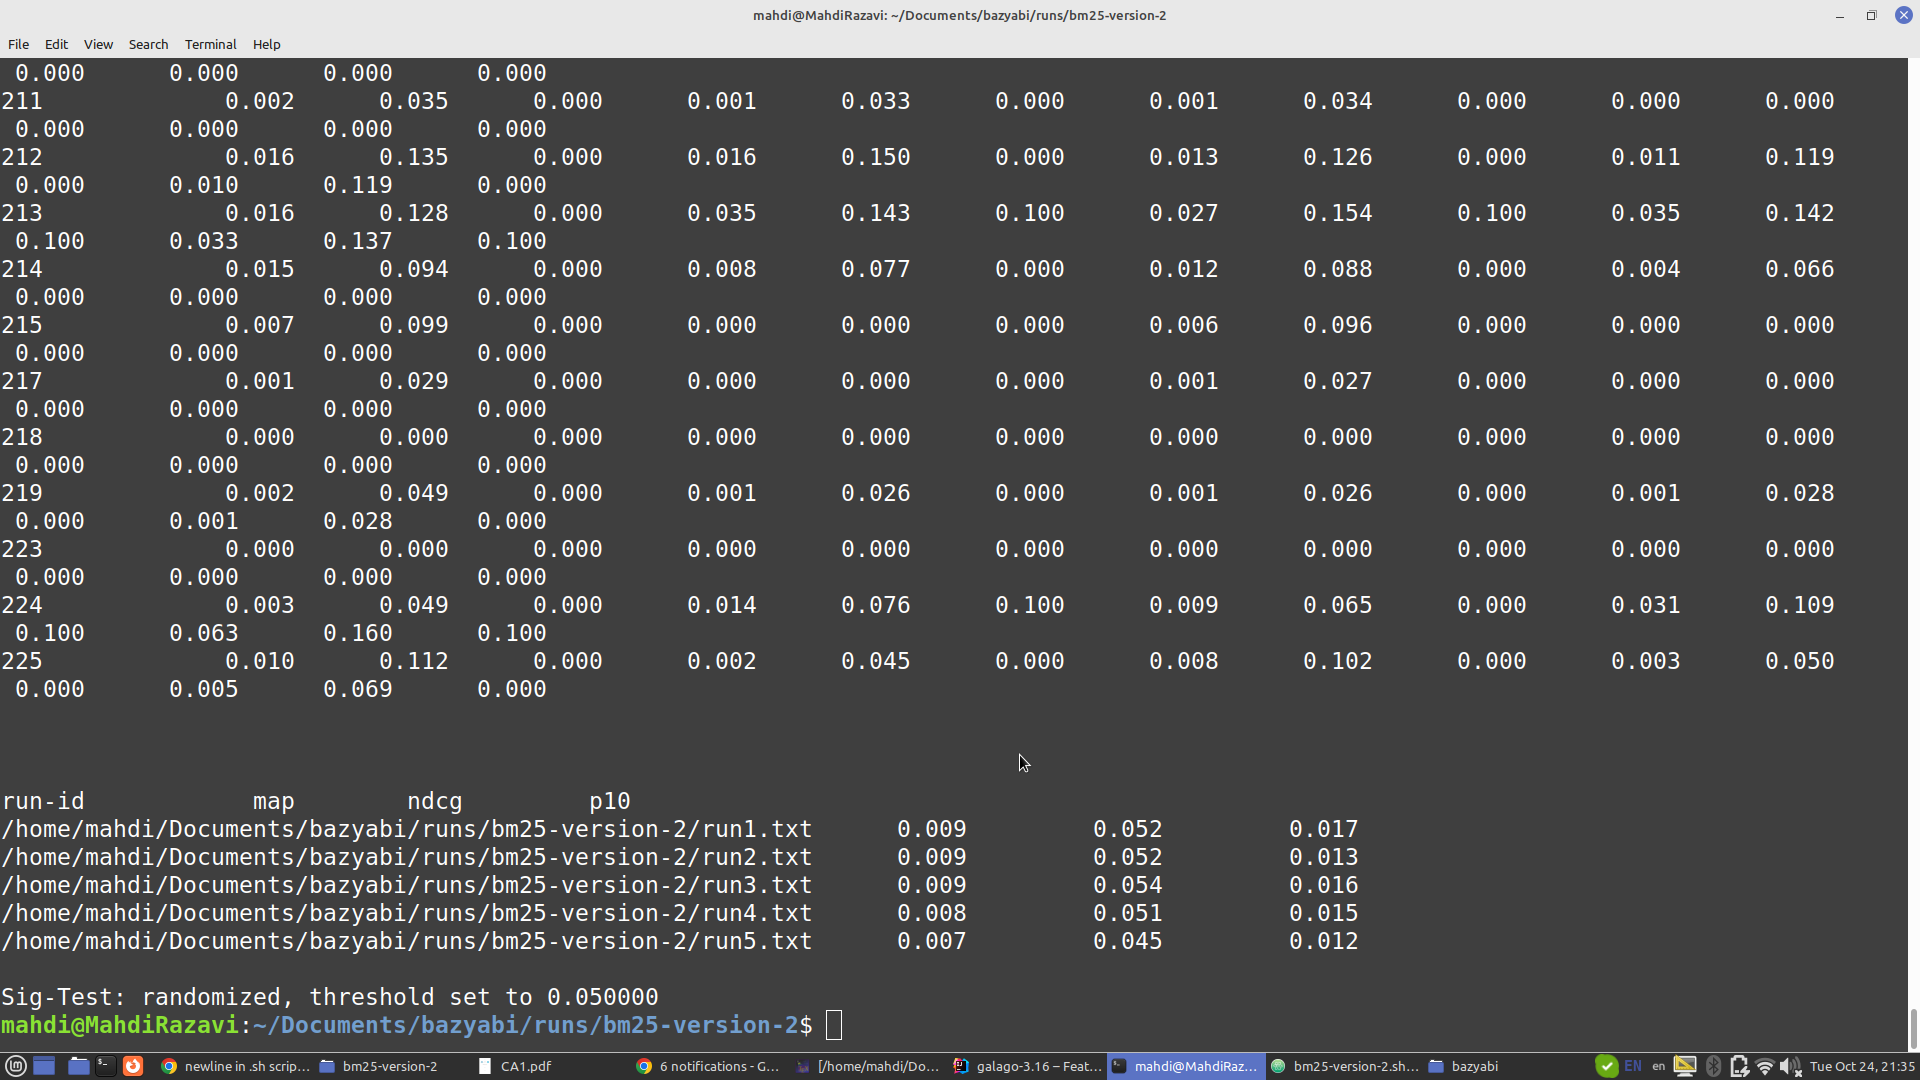
\includegraphics[width=0.9\textwidth]{IR1/images/V2.png}
% \caption{ت هستند.}
\caption{تابع امتیازدهی دوم}
\end{figure}

\begin{boxM}
    با توجه به ضابطه تابع امتیازدهی به اسناد ، باز متوجه خواهیم شد که ضابطه مستقل از پارامتر
    \lr{b}
    می‌باشد.

    از تغییرات متغیر
    \lr{k}
    متوجه خواهیم شد که هر چه میزان این متغیر به ۱ نزدیک‌تر باشد ، 
    نتایج جستجو بهتر خواهد بود.

    زیرا که تاثیر فراوانی عبارات مشترک را کمتر خواهد کرد .
\end{boxM}

\newpage

\begin{figure}[h]
    \centering
    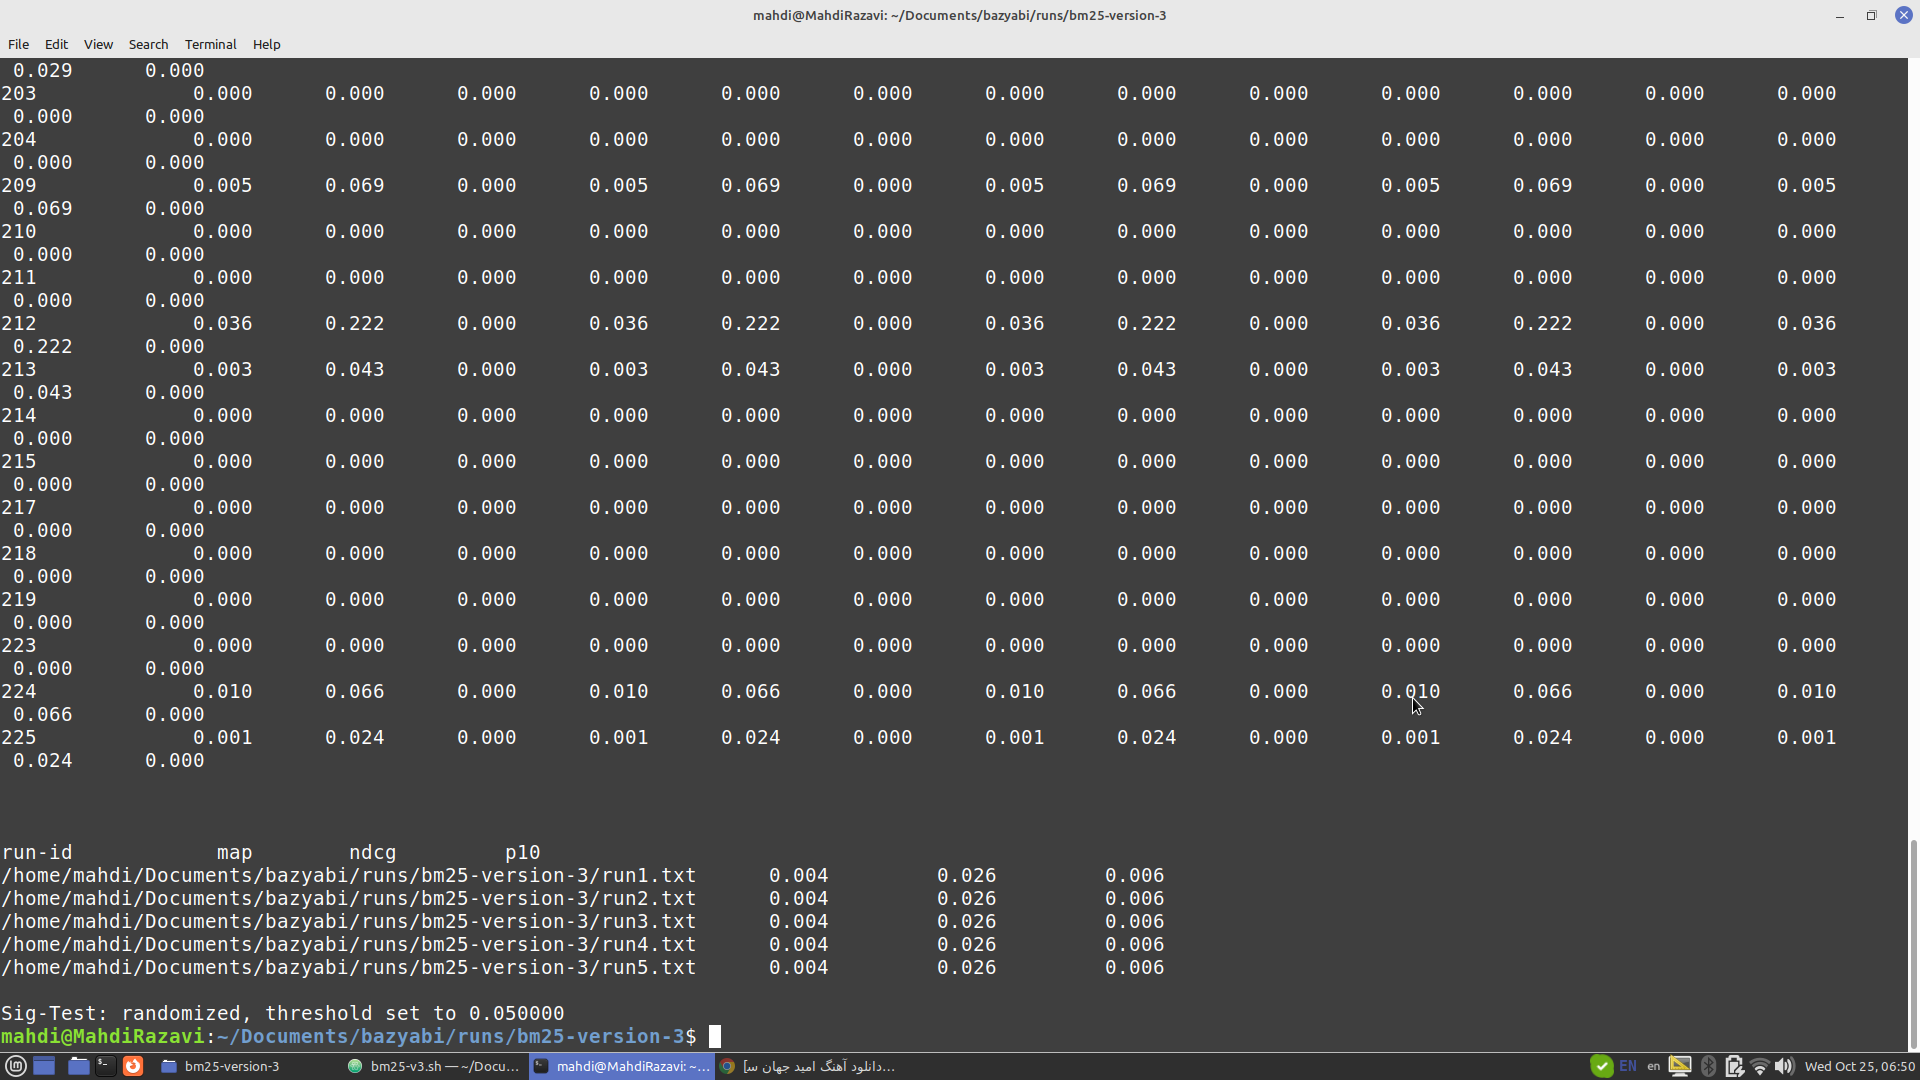
\includegraphics[width=0.8\textwidth]{IR1/images/V3.png}
    \caption{نتایج مرتب‌سازی با تابع امتیازدهی ۳}
    \label{fig:enter-label}
\end{figure}

\begin{boxM}
    این روش نیز مانند روش اول 
    مستقل از پارامترهای 
    \lr{b}
    و 
    \lr{k}
    خواهد بود.

    نتایج همگی مشابه هم خواهند بود.
    این روش در تلاش است که تاثیر طول اسناد ، تاثیر کمتری در نتایج نهایی داشته باشد.
    چرا که طبیعتا هر چه طول سند بیشتر باشد ، احتمال مرتبط بودن پرس‌وجو با آن بیشتر خواهد بود.
\end{boxM}

\newpage

\begin{figure}
    \centering
    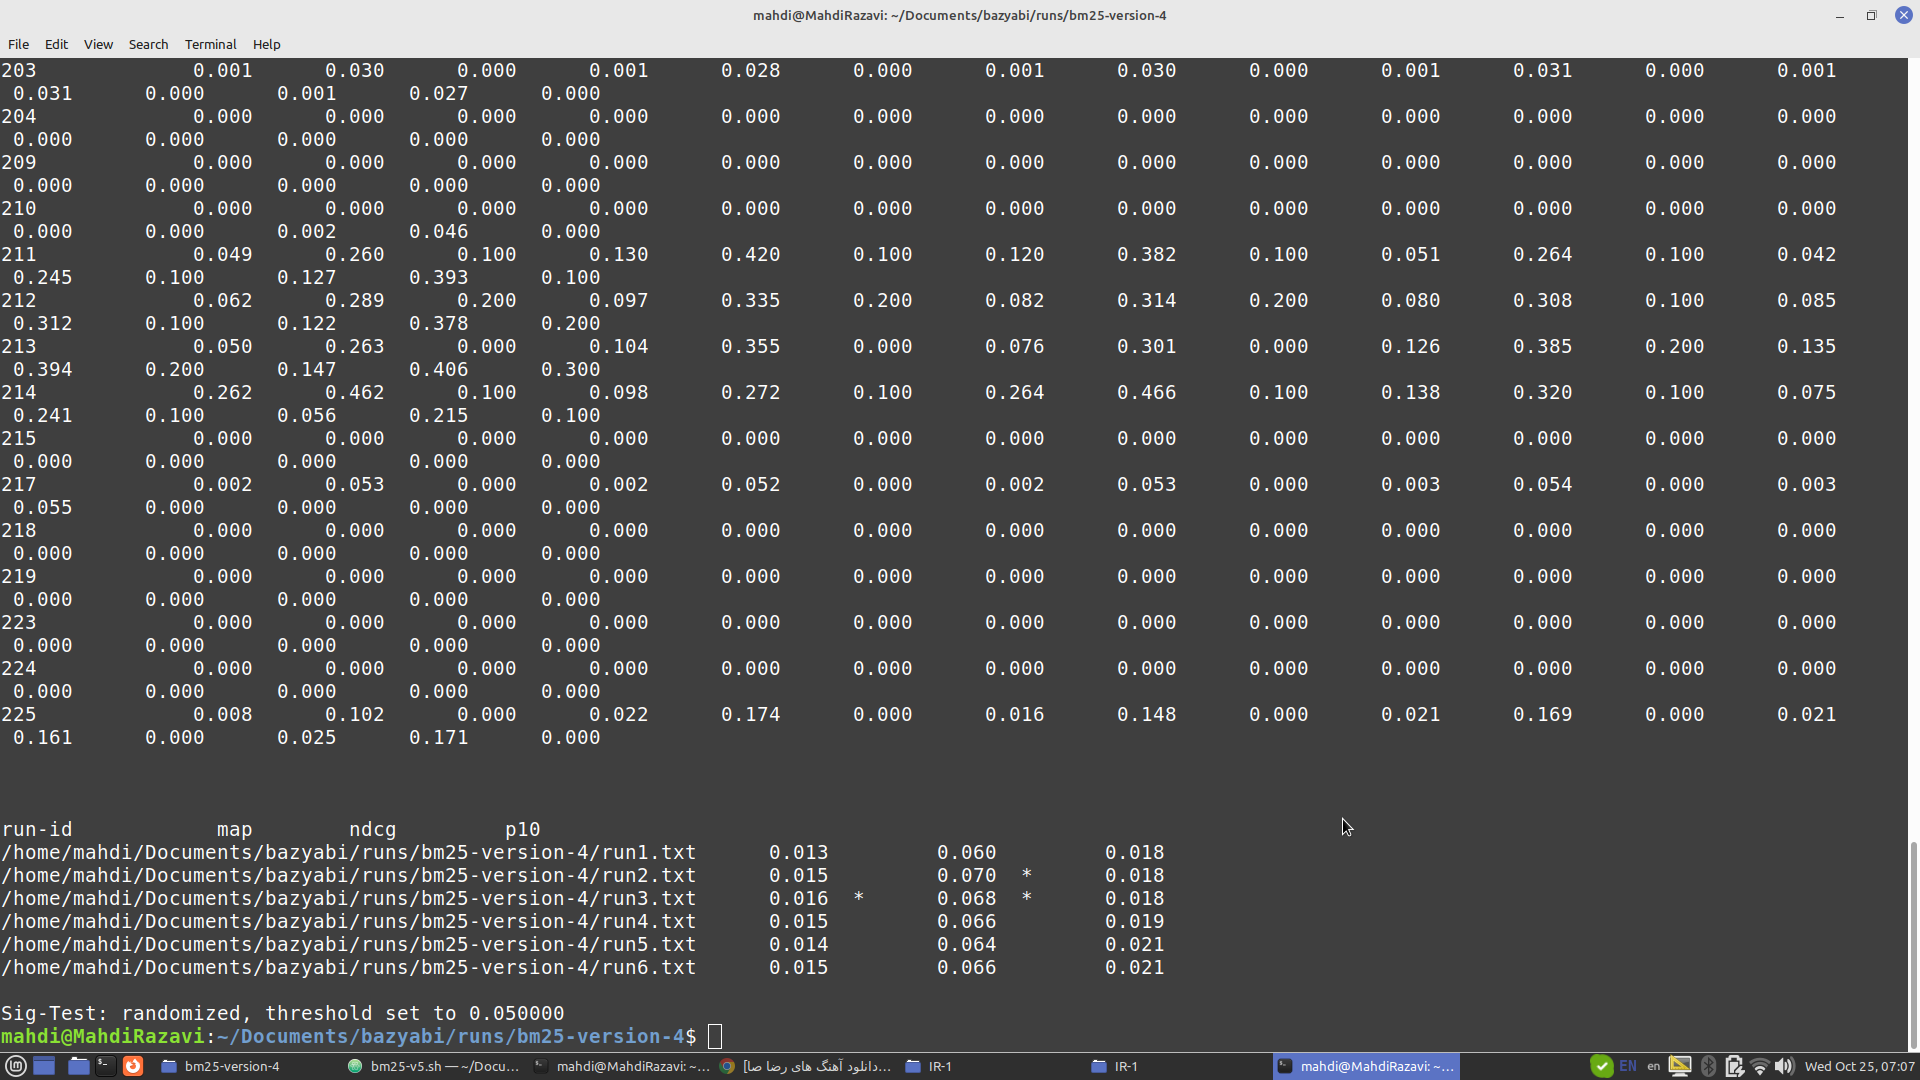
\includegraphics[width=0.8\textwidth]{IR1/images/V4.png}
    \caption{نتایج مرتب‌سازی با تابع امتیازدهی ۴}
    \label{fig:enter-label}
\end{figure}

\begin{boxM}
    همانطور که در تصویر مشخص است ، بهترین نتایج مربوط به اجرای شماره ۳ می‌باشد.
    در این اجرا ما پارامترهای زیر را داشته‌ایم :
    \begin{equation*}
        k = 1.75 , b = 0.52
    \end{equation*}
    
    
\end{boxM}

\newpage

\begin{figure}
    \centering
    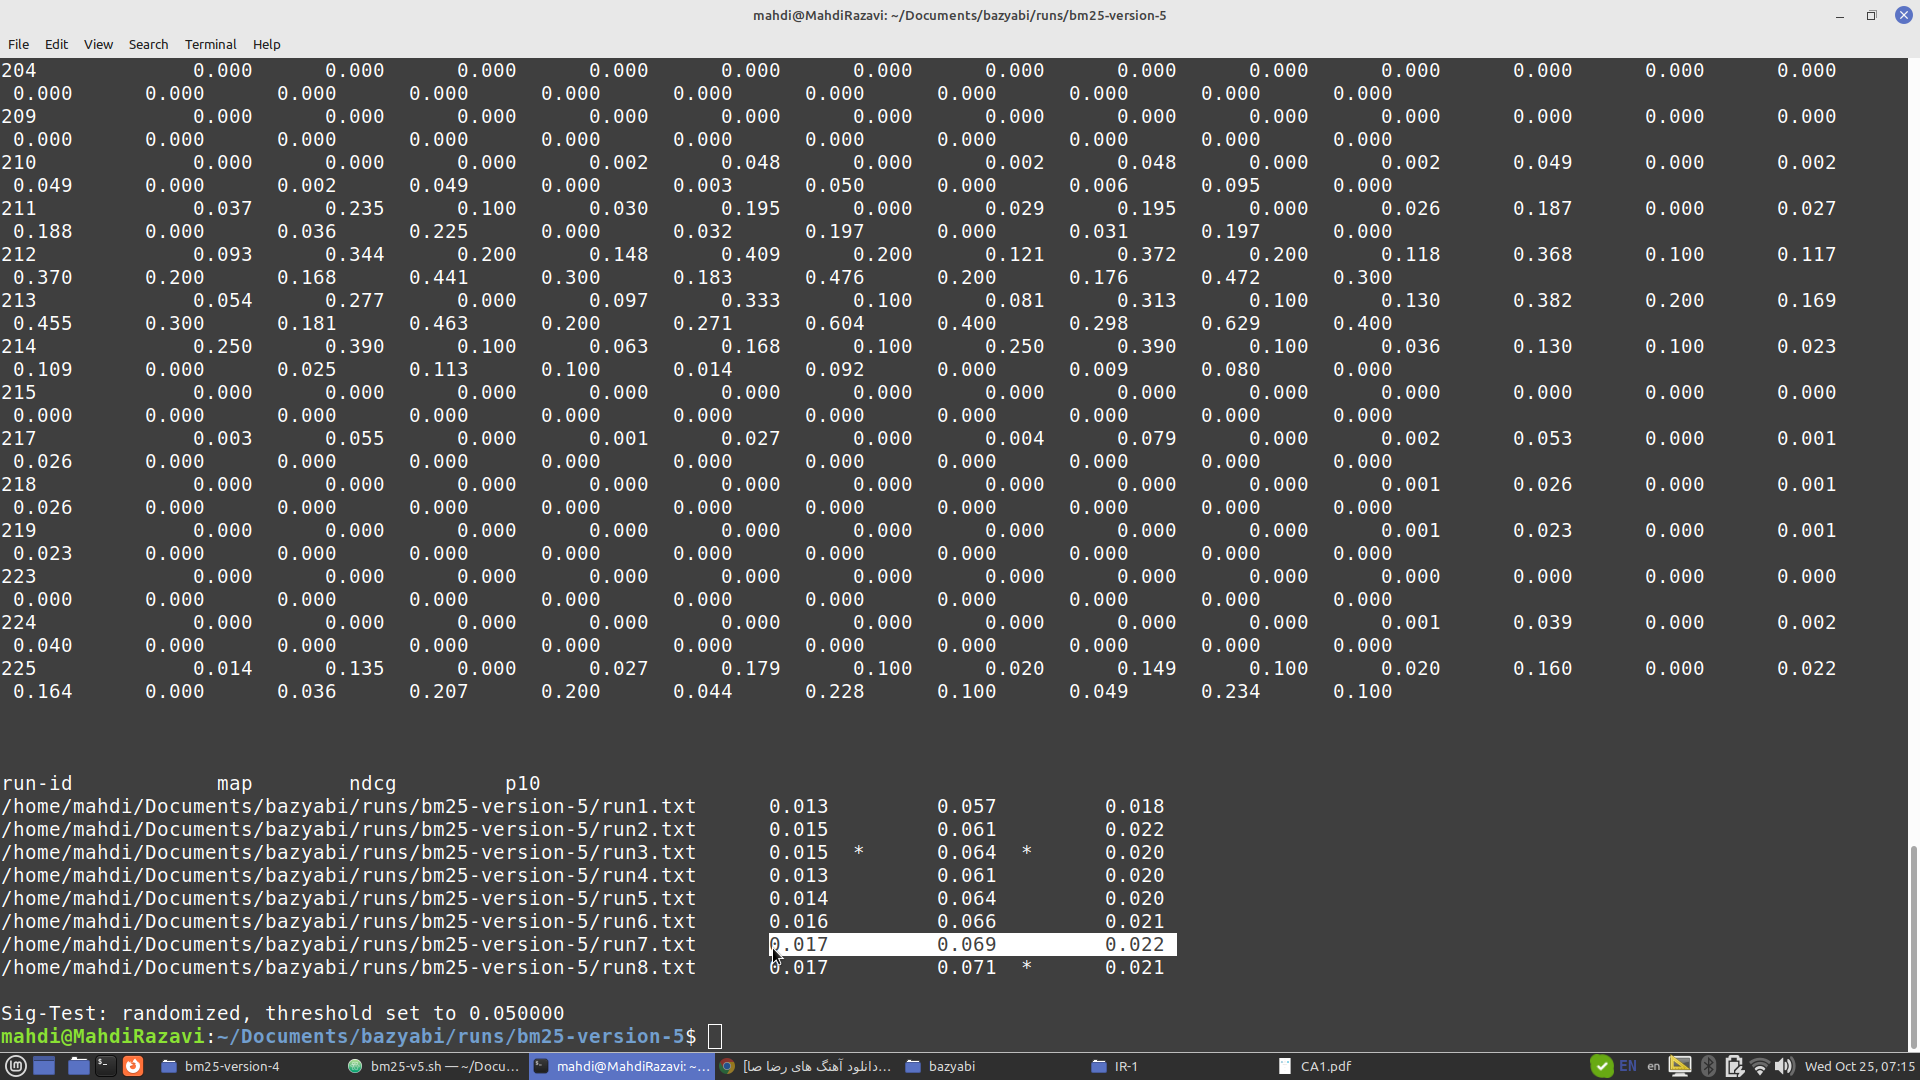
\includegraphics[width=0.8\textwidth]{IR1/images/V5.png}
    \caption{نتایج مرتب‌سازی با تابع امتیازدهی ۵}
    \label{fig:enter-label}
\end{figure}

\begin{boxM}
    در این روش طبق تصاویر نتایج مشاهده‌شده ، بهترین اجرای ما ،اجرای شماره ۷ خواهد بود.
    پارامترهای این اجرا عبارت خواهند بود از :
    \begin{equation*}
        b = 0.92 , k = 18.75
    \end{equation*}

    از این آزمایش نتیجه می‌گیریم که با افزایش مقدار 
    \lr{k}
    احتمال موفقیت‌آمیزتر بودن آزمایش ما بیشتر است.

    زیرا با افزایش این مقدار ، تاثیر عبارات بسیار تکرارشونده خیلی کم می‌شود.
\end{boxM}

\newpage

\begin{figure}
    \centering
    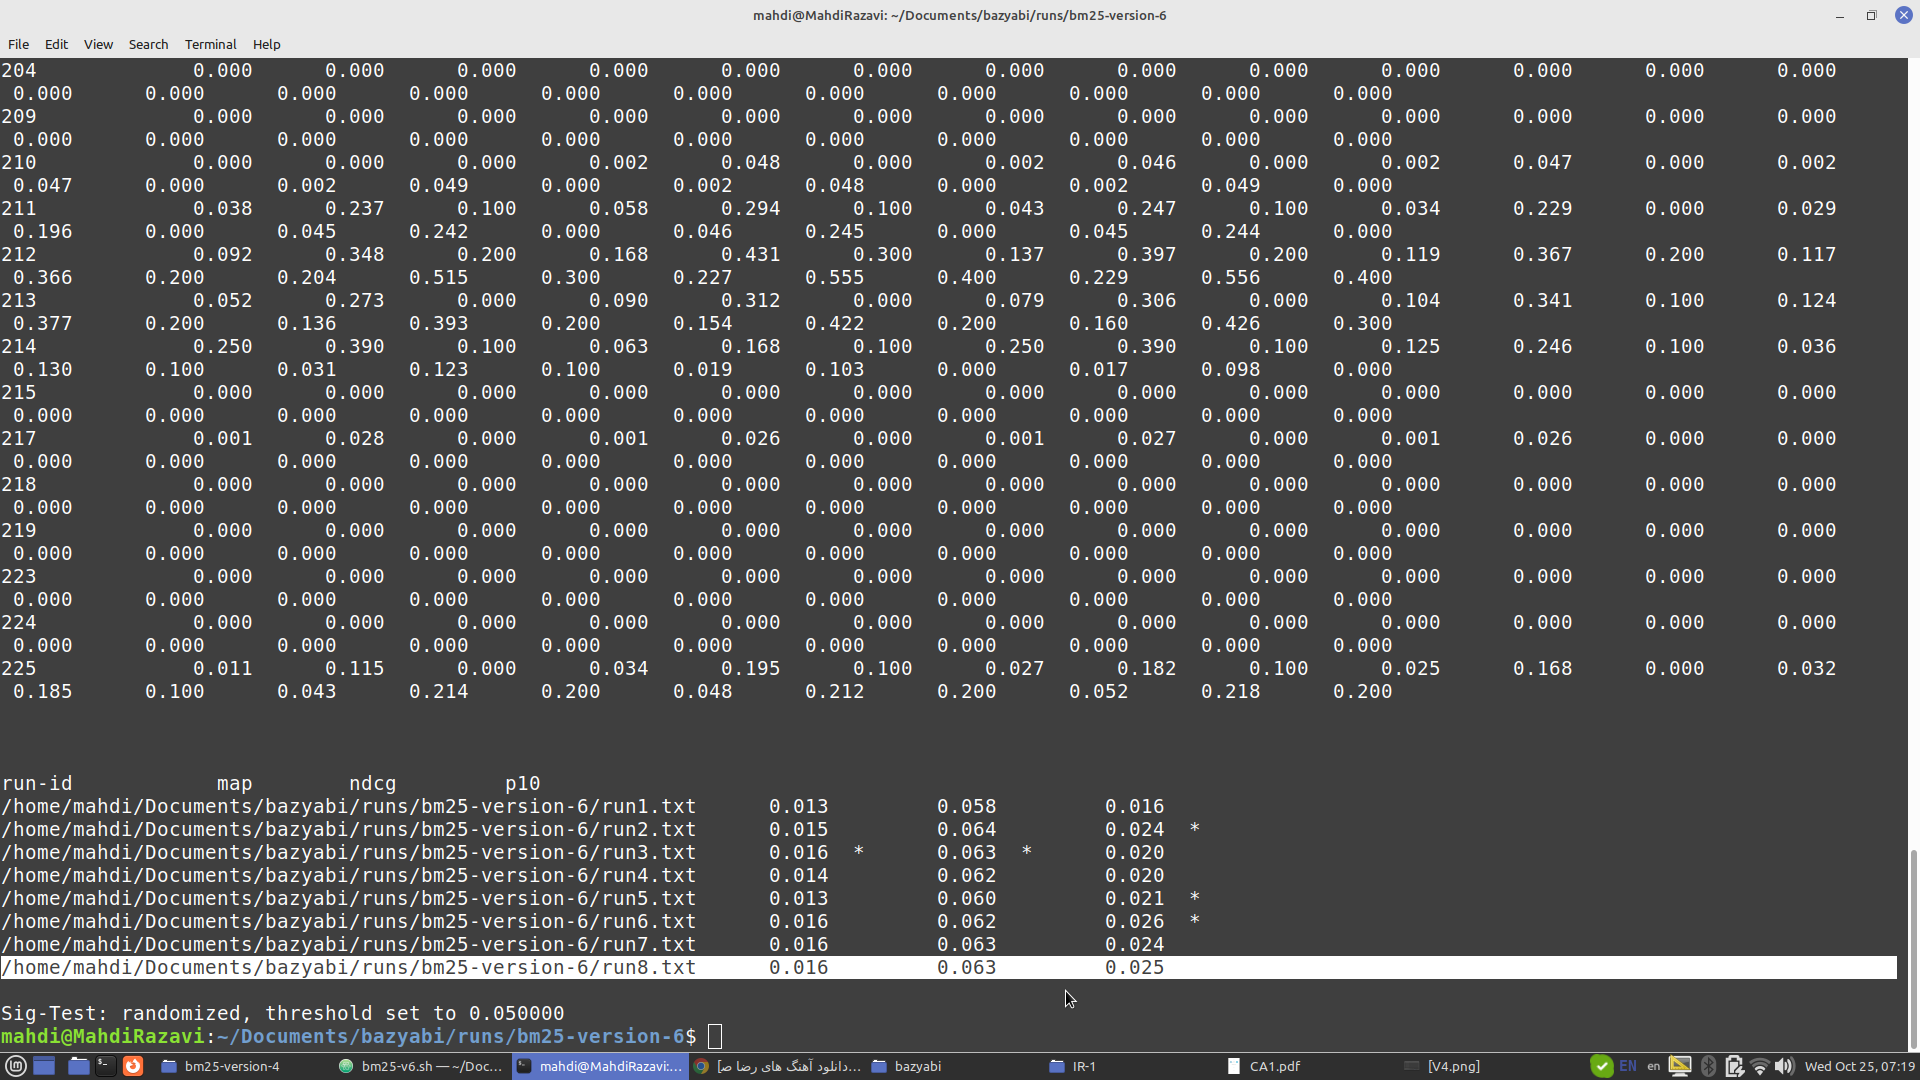
\includegraphics[width=0.8\textwidth]{IR1/images/V6.png}
    \caption{نتایج مرتب‌سازی با تابع امتیازدهی ۶}
    \label{fig:enter-label}
\end{figure}

\begin{boxM}
    در این آزمایش با تغییر پارامترها 
    بهترین آزمایش را در اجرای ۸ ام داشتیم.

    \begin{equation*}
        k=8.75  , b=0.82
    \end{equation*}

    تاثیر افزایش پارامتر
    \lr{b}
    که بین صفر  و یک است در این آزمایش به وضوح نشان‌داده شده است.
    
\end{boxM}

\newpage

\begin{figure}
    \centering
    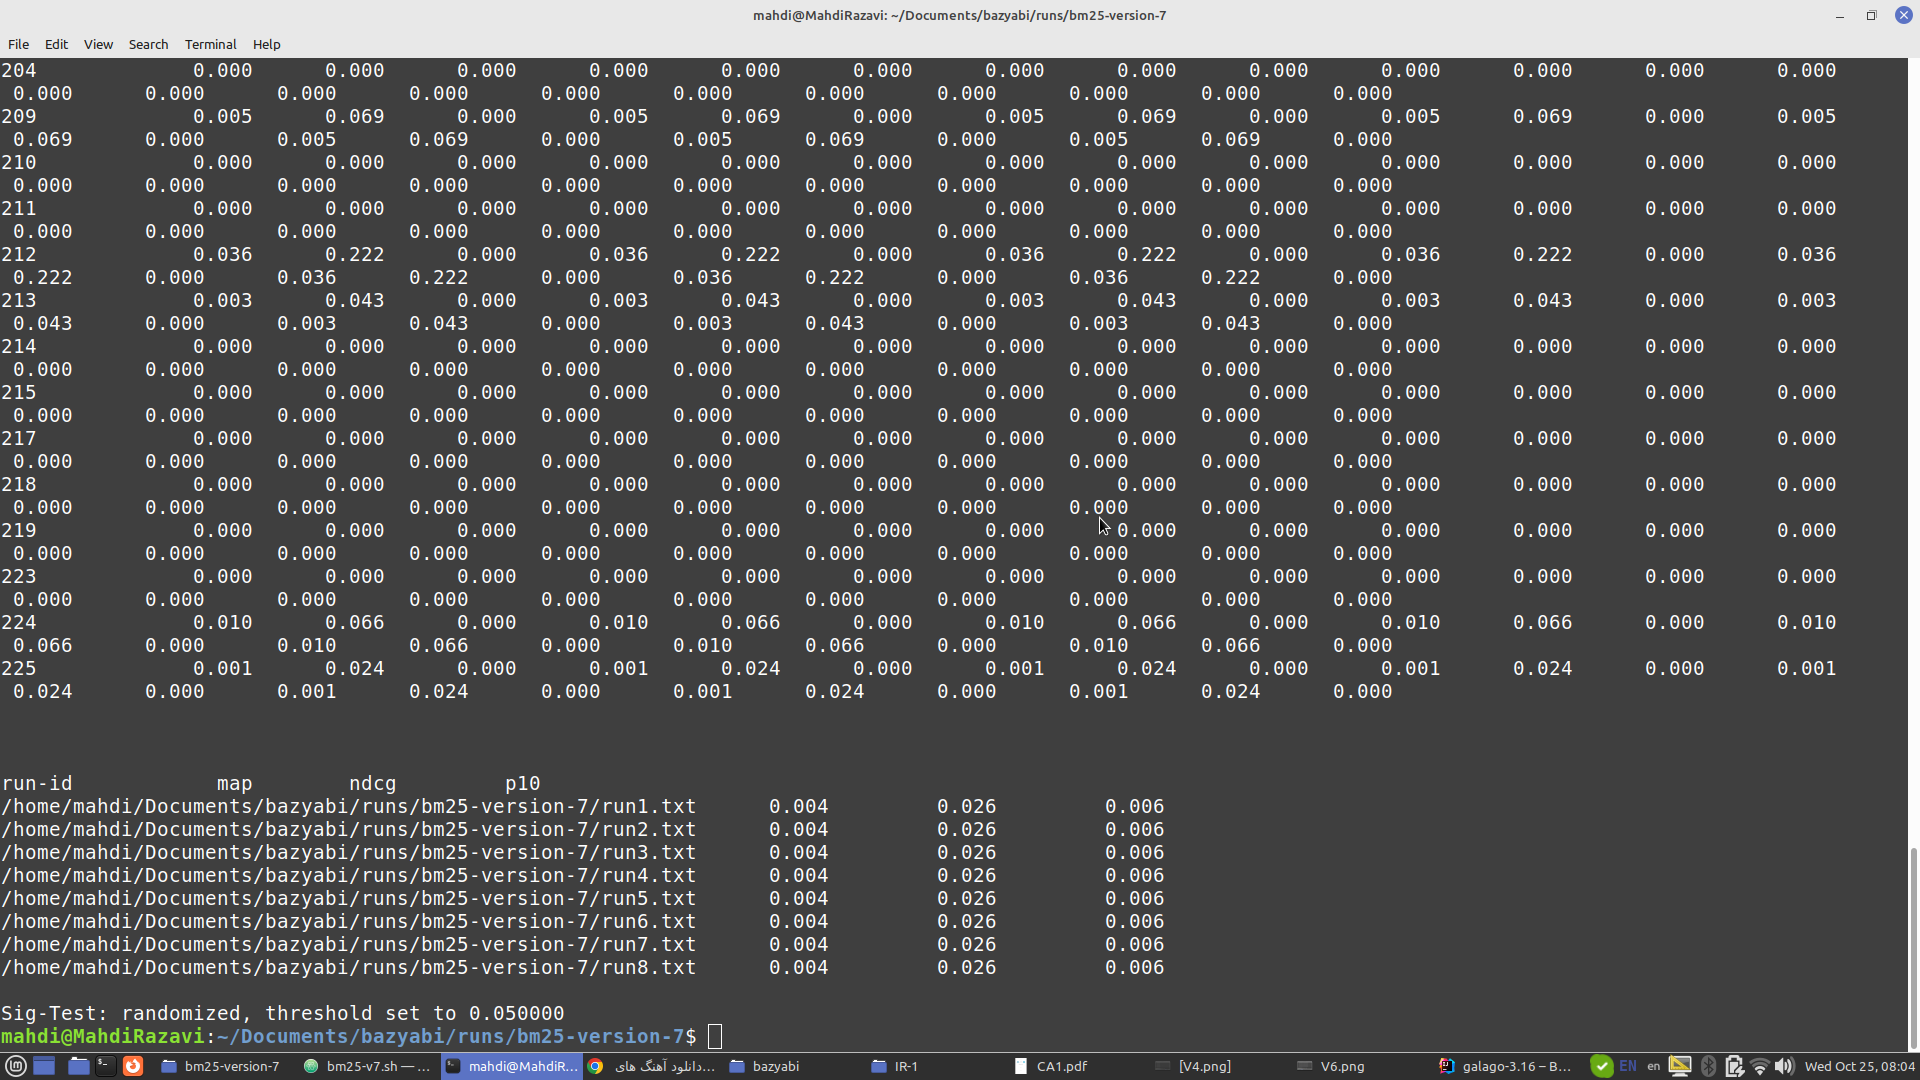
\includegraphics[width=0.8\textwidth]{IR1/images/V7.png}
    \caption{نتایج مرتب‌سازی با تابع امتیازدهی ۷}
    \label{fig:enter-label}
\end{figure}

\begin{boxM}
    متاسفانه تغییری در نتایج آزمایش‌ها مشاهده نشد.
    چون که آزمایش‌ها مستقل از
    \lr{k}
    می‌باشند ، 
    متوجه خواهیم شد که تاثیر پارامتر
    \lr{b}
    نیز بسیار ناچیز است.
\end{boxM}